	\section{Domain} 
		\subsection{Domainmodel}
		
		
		
		\subsection{Task-Vorlagen strukturierung}
			Es gibt verschiedene Möglichkeiten, 
			Benutzer eine Strukturierung von Task-Vorlagen anzubieten.
			Task-Templates können selbst in eine Struktur gebracht werden, 
			oder durch externe Strukturen geordnet werden.
		
			\begin{figure}[H]
				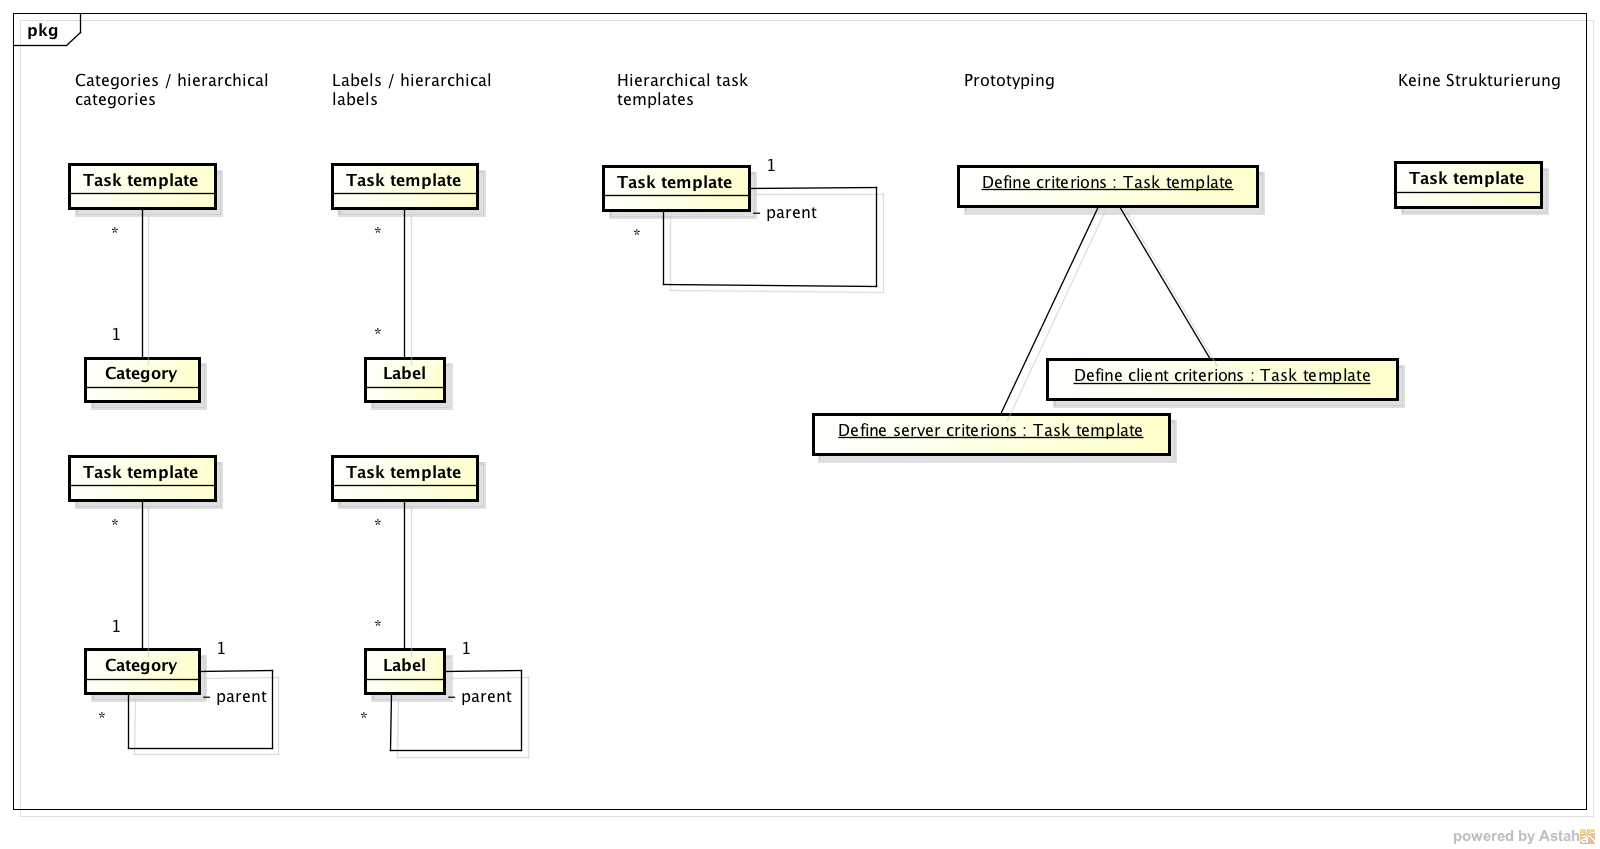
\includegraphics[width=\textwidth]{architecture/media/img/taskTemplateStructure.png}
				\centering
				\caption{Strukturierungsmöglichkeiten von Tasks}
				\label{fig:taskTemplateStructure}
			\end{figure}
			
		\decision{
			\decisionHeader{D-S-1}{Task-Vorlagen Strukturierung}{Architecture}{Domain}
		}{
			\decisionContent{Nicht hierarchische Kategorien, Smart Filters}
			{Welches Konzept soll zur Strukturierung von Task-Vorlagen eingesetzt werden?}
			{}{Benutzer sollen einfach und schnell erstellte Task-Vorlagen wieder finden.}
			{
				\begin{description}
					\item[Keine Strukturierung] \
						\begin{description}
							\item[Vorteile] Einfach zu implementieren, einfach verständlich für den Benutzer
							\item[Nachteile] Bei vielen Task-Vorlagen unübersichtlich, führt zu doppelten Task-Vorlagen da existierende nicht gefunden werden. 
						\end{description}
						
					\item[Labels/Hierarchische Labels] \
						Versehen der Elemente mit einem oder mehreren Labels. Benutzer können nach Labels suchen oder Filtern, um Vorlagen anzuzeigen.	
						\begin{description}
							\item[Vorteile] Einfach verständlich für den Benutzer
							\item[Nachteile] Benutzer könnten zu Faul sein, Labels anzulegen und zuzuordnen da es aufwändiger ist als Kategorisieren
						\end{description}
					
					\item[Direkte Hierarchisierung der Task-Vorlagen] \
						Elemente werden direkt mit Elternelementen verknüpft und bilden einen hierarchischen Baum.	
						\begin{description}
							\item[Vorteile] Einfach zu implementieren
							\item[Nachteile] Schwer verständlich für den Benutzer da die Hierarchisierung unter Umständen nicht mit dem Workflow zusammenpasst
						\end{description}
					
					\item[Prototyping statt Strukturierung] \
						Elemente erben Funktionalität von einander, statt strukturiert zu werden.
						\begin{description}
							\item[Vorteile] Verringert die Anzahl Task-Vorlagen massiv, da Eigenschaften vererbt werden können
							\item[Nachteile] Schwieriger umzusetzen, schwieriger zu verstehen für Benutzer
						\end{description}					
				\end{description}
			}
			{
				Kategorien erlauben eine Strukturierung auf einfache Weise. 
				Für diesen Anwendungsfall reichen nicht hierarchische aus, 
				da Task-Vorlagen wiederverwendet werden und daher die Anzahl Task-Vorlagen nicht Grössen erreichen, 
				die hierarchische Kategorien erfordern würden. 
				Zudem sind hierarchische Strukturen komplizierter um Vorlagen zu finden und aufwändiger umzusetzen.
				
				Smart Filter ergänzen Kategorien optimal und ermöglichen das schnelle Finden anhand von Eigenschaften,
				die über Kategorien hinausgehen.
			}
			{}
			{}
			{}
		}
		
		
		\subsection{Verknüpfungen von Task-Vorlagen und Entscheidungs-Vorlagen}
			Wissensproduzenten können Task-Vorlagen zu Entscheidungs-Vorlagen zuordnen.
			Dabei kann und soll auch eine Task-Vorlage an verschiedene Entscheidungs-Vorlagen zugeordnet werden können.
			Ebenso können Entscheidungs-Vorlagen natürlich mehrere Task-Vorlagen zugeordnet erhalten.
			
			\subsubsection{Arten der Zuordnung}
				Task-Vorlagen können mit Entscheidungs-Vorlagen auf zwei Arten verknüpft werden:
				\begin{enumerate}
					\item Sie können dann fällig werden, wenn eine Entscheidung getroffen wurde (operativer Task).
					\item Eine Task-Vorlage dient dazu, Entscheidungen zu treffen (Entscheidungstask).
				\end{enumerate}
				Auf die Task-Vorlagen selbst hat dies keinen Einfluss, sie sind unabhängig davon. 
				Ob es sich um einen operativen Task oder einen Entscheidungstask handelt hängt nur davon ab,
				ob die Task-Vorlage mit einer Entscheidung (Node) oder einer Option einer Entscheidung (Subnode) des Entscheidungsbaumes verknüpft ist.

			\subsubsection{Übertragung in \ppt}
				Aus diesen Task-Vorlagen werden beim Übertag in ein \ppt\ Tasks generiert.
				Task-Vorlagen sind generisch, da Änderungen auch alle verknüpften Entscheidungs-Vorlagen betreffen sollen.
				Aus diesem Grund werden Task-Vorlagen bei der Zuordnung verknüpft und nicht kopiert.
				
				\begin{figure}[H]
					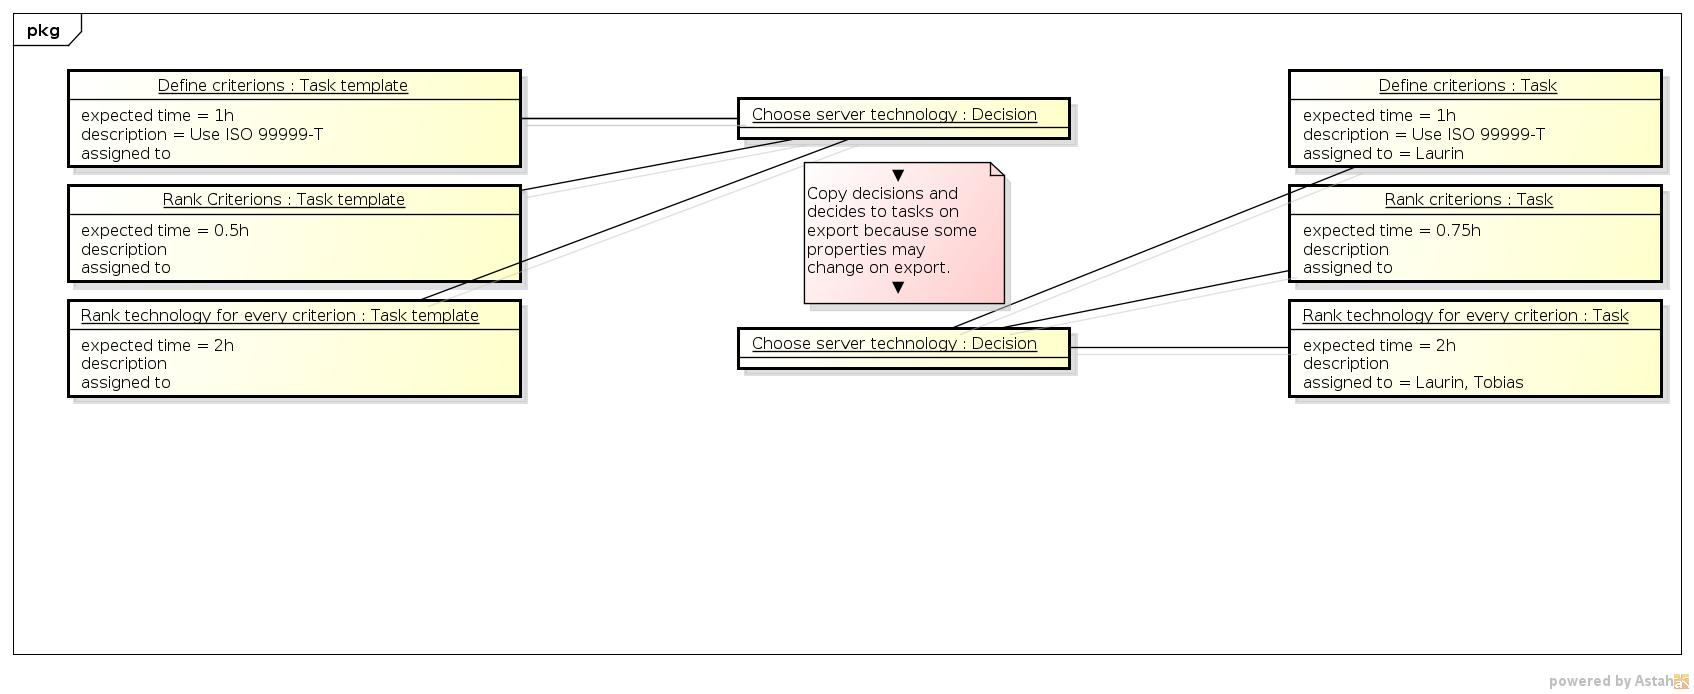
\includegraphics[width=\textwidth]{architecture/media/img/DecisionTaskRelation.jpg}
					\centering
					\caption{Übertragen von Entscheidungen und Task-Vorlagen}
					\label{fig:DecisionTaskRelation}
				\end{figure}
				
				Beim Übertragen werden aus Task-Vorlagen (konkrete) Tasks.
				Auch Entscheidungen werden zu Tasks übertragen, da \ppt's keine Entscheidungen kennen.
				Mit Entscheidungen verknüpfte Tasks werden entsprechend zu Sub-Tasks.
				
				Benutzer wollen bei der Übertragung ins \ppt\ die von der Task-Vorlage vorgegebenen Werte möglicherweise anpassen, wie z.B. den erwarteten Aufwand für den Task.
				Daher ist es sinnvoll, die Eigenschaften der Task-Vorlagen in die (konkreten) Tasks zu kopieren, anstatt sie lediglich zu verknüpfen.
				Gleiches gilt für Entscheidungen. Würde jemand im CDAR diese verändern oder Löschen, so würde dies die History zerstören.
			
		
		\subsection{Tasktransmission Workflow}
			Aus Task-Vorlagen erzeugte Tasks müssen zur Übertragung in ein Projektmanagementtool
			Tool spezifisch umgewandelt werden. Dazu werden "`Processors"' eingesetzt.
			"`Processors"' stellen kleine Funktionalitäten dar, die Daten umwandeln, wie z.B. "`Date processors"', die Daten umwandeln, "`Issue type processors"', die Issuetypes konvertieren, "`User processors"', die Relationen zu Benutzern so umwandeln, das das Projektplanungstool den User korrekt verknüpfen kann oder "`Conditional processors"' und "`Option processors"', die Bedingungen verarbeiten.
			Ebenfalls denkbar ist ein Processor, der Felder aggregieren kann und damit z.B. nicht gemappte Felder in die Beschreibung überführen kann.
			
			\begin{figure}[H]
				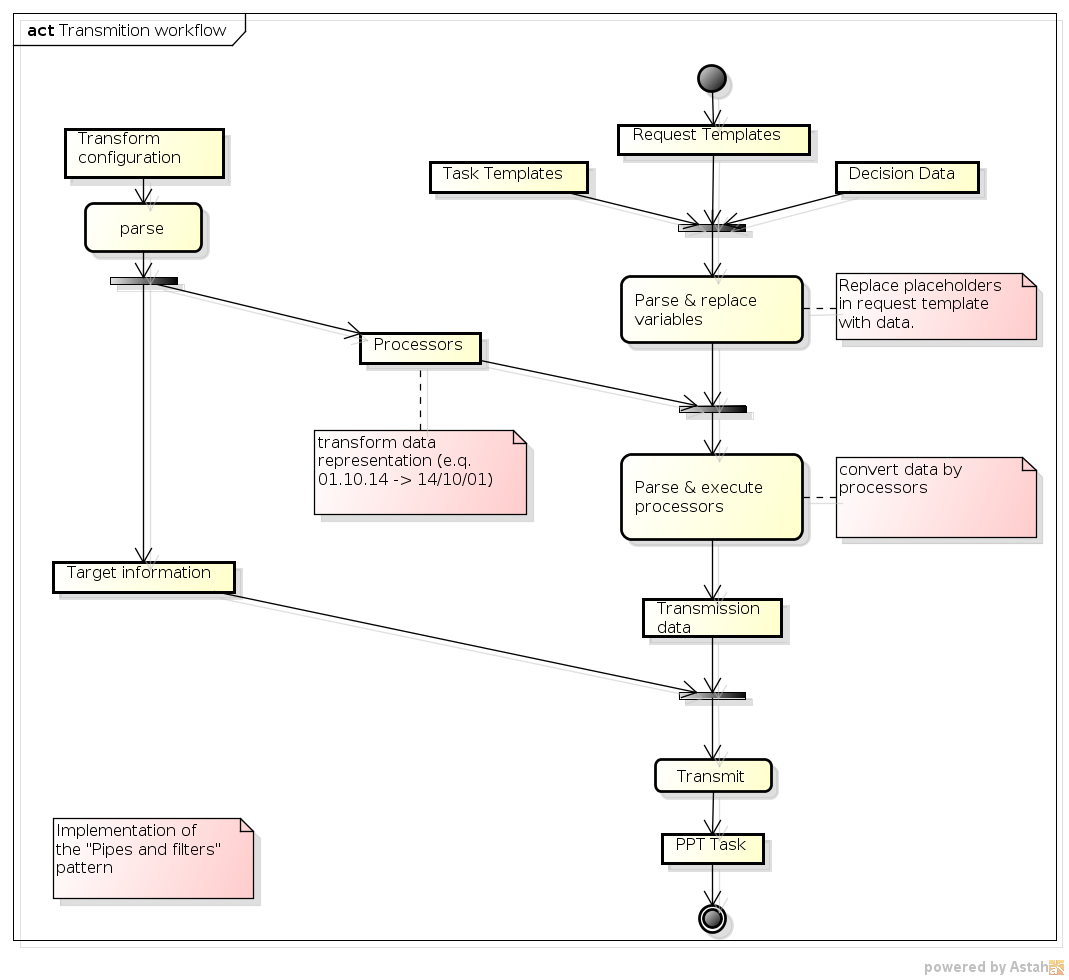
\includegraphics[width=\textwidth]{architecture/media/img/transmissionWorkflow.png}
				\centering
				\caption{Übertragen von Tasks}
				\label{fig:transmissionWorkflow}
			\end{figure}
			
			Der komplette Tasktransmission Workflow soll auf dem Client durchgeführt werden und nicht auf dem Server. Grund dafür sind einerseits die Problematik, 
			das sich der \eeppi\ Server in einer Zone befinden kann, 
			die ihm keinen direkten Zugriff auf den Projektmanagementtool-Server erlaubt,
			andererseits schränkt die Wahl der Servertechnologie die Möglichkeiten für dynamische Processors ein, während die Client Technologie dies ermöglicht.
			
			Im Laufe der Erarbeitung dieses Workflows wurde auch darüber nachgedacht, 
			was mit noch nicht gemappten Eigenschaften passieren soll. 
			Die ursprüngliche Entscheidung, diese in Listenform in die Beschreibung des Tasks
			überzuführen wurde durch das flexible Mapping obsolete, 
			weil einerseits dazu in jedem Fall bekannt sein muss, welches Feld das Beschreibungsfeld ist 
			und andererseits der Administrator dazu selbst einen Processor definieren kann.
			Womit die Entscheidung darüber bei ihm bleibt und nicht von uns vorgegeben wird.
		
		
		\subsection{Mapping method}
		\decision{
			\decisionHeader{D-S-2}{Mapping method}{Architecture}{Domain}
		}{
			\decisionContent{Konfiguration/Block}
			{Wie sollen Mappingkonfigurationen erstellt werden?}
			{}
			{}
			{
				\begin{description}					
					\item[Hierarchische/Element basierte Konfiguration] \
					Das Mapping wird durch das Anlegen von verknüpften Elementen erzeugt.
					\begin{description}
						\item[Vorteile] Gegebene Validierung durch die Struktur, kein Parser notwendig
						\item[Nachteile] Aufwändiger umzusetzen, insbesondere das UI, weniger flexibel
					\end{description}
				\end{description}
			}
			{Eine Textblock-basierte Konfiguration erhöht zwar die Fehlermöglichkeiten für den Administrator,
			ermöglicht diesem jedoch grössere Flexibilität und damit ein Abdecken einer grösseren Bandbreite an Projektplanungstools.}
			{}
			{}
			{}
		}
		
		Der Ablauf für einen Administrator sieht entsprechend wie folgt aus:
		\begin{enumerate}
			\item Projektplanungstool definieren
			\item Taskeigenschaften erstellen
			\item Mapping Taskeigenschaften -> Projektplanungstool erstellen
		\end{enumerate}
		
		
		\subsection{EEPPI Domain}
			
				
		
		\subsection{Communication}